% ---
% title: Denoising Diffusion Models, Derived
% author: Mejistus
% ---
\newcommand{\E}{\mathbb{E}}
\newcommand{\N}{\mathcal{N}}
\newcommand{\KL}{D_{\mathrm{KL}}}
\newcommand{\abar}{\bar\alpha}
\usetikzlibrary{arrows.meta,positioning}

\begin{abstract}
Diffusion models generate data by learning to undo a fixed process that gradually turns data into Gaussian noise.
This note derives the denoising diffusion probabilistic model (DDPM) from first principles, with every step written out: the closed-form forward marginals, the variational bound and its decomposition into Gaussian KL terms, the Gaussian posterior of the forward process, and the reparameterisation that turns the bound into a noise-prediction loss.
We then show that the optimal noise predictor is a scaled score function (Tweedie's formula), which connects DDPM to denoising score matching, and we derive deterministic DDIM sampling and the continuous-time SDE limit from the same quantities.
\end{abstract}

\section{Introduction}\label{sec:intro}
A diffusion model~\cite{sohl2015,ho2020} pairs two Markov chains.
The \emph{forward} chain $q$ adds a small amount of Gaussian noise at each of $T$ steps until nothing of the data is left; it has no parameters.
The \emph{reverse} chain $p_\theta$ starts from pure noise and removes it step by step; it is the generative model, and learning it is the whole problem (Figure~\ref{fig:chain}).
Because each forward step is small, each reverse step is close to Gaussian, so the model only has to learn a mean.

This note makes the following points, each with a complete derivation:
\begin{itemize}
  \item the forward process has a closed-form marginal $q(x_t \mid x_0)$ at every step (Proposition~\ref{prop:marginal}), so training never simulates the chain;
  \item the variational bound splits into one KL divergence per step (Proposition~\ref{prop:elbo}), each between Gaussians and so in closed form, because the forward posterior $q(x_{t-1} \mid x_t, x_0)$ is Gaussian (Proposition~\ref{prop:posterior});
  \item predicting the added noise is equivalent to predicting the score $\nabla_x \log q_t(x)$ (Proposition~\ref{prop:tweedie}), which is why diffusion models and score-based models~\cite{song2019,song2021sde} are the same family;
  \item the same trained network supports deterministic sampling (Section~\ref{sec:ddim}) and has a stochastic differential equation as its continuous-time limit (Section~\ref{sec:sde}).
\end{itemize}

\begin{figure}[t]
  \centering
  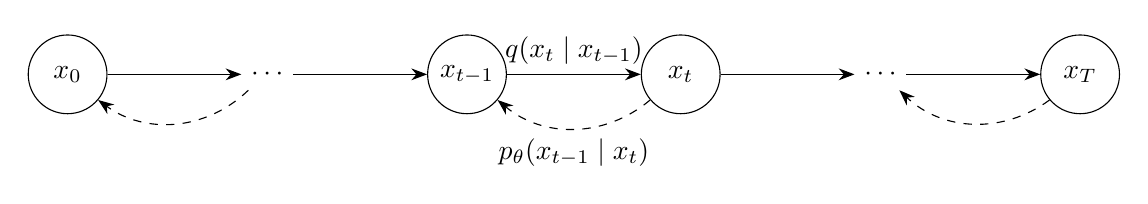
\begin{tikzpicture}[node distance=17mm, >={Stealth[length=2mm]},
                      st/.style={draw, circle, minimum size=10mm, inner sep=0pt}]
    \node[st] (x0) {$x_0$};
    \node[right=of x0] (d1) {$\cdots$};
    \node[st, right=of d1] (xs) {$x_{t-1}$};
    \node[st, right=of xs] (xt) {$x_t$};
    \node[right=of xt] (d2) {$\cdots$};
    \node[st, right=of d2] (xT) {$x_T$};
    \draw[->] (x0) -- (d1);
    \draw[->] (d1) -- (xs);
    \draw[->] (xs) -- node[above] {$q(x_t \mid x_{t-1})$} (xt);
    \draw[->] (xt) -- (d2);
    \draw[->] (d2) -- (xT);
    \draw[->, dashed] (xt) to[bend left=40] node[below] {$p_\theta(x_{t-1} \mid x_t)$} (xs);
    \draw[->, dashed] (xT) to[bend left=40] (d2);
    \draw[->, dashed] (d1) to[bend left=40] (x0);
  \end{tikzpicture}
  \caption{The two chains. The forward process $q$ (solid) is fixed and adds noise; the reverse process $p_\theta$ (dashed) is learned and removes it.}\label{fig:chain}
\end{figure}

\section{The forward process}\label{sec:forward}
Fix a variance schedule $\beta_1, \dots, \beta_T \in (0, 1)$ and define
\begin{equation}\label{eq:forward-step}
  q(x_t \mid x_{t-1}) = \N\!\left(x_t;\ \sqrt{1-\beta_t}\,x_{t-1},\ \beta_t I\right),
  \qquad q(x_{1:T} \mid x_0) = \prod_{t=1}^{T} q(x_t \mid x_{t-1}).
\end{equation}
Scaling the mean by $\sqrt{1-\beta_t}$ keeps the variance bounded: if $x_{t-1}$ has unit variance, so does $x_t$.
Throughout we write
\begin{equation}\label{eq:alphas}
  \alpha_t = 1 - \beta_t, \qquad \abar_t = \prod_{s=1}^{t} \alpha_s .
\end{equation}

\begin{proposition}[Closed-form marginals]\label{prop:marginal}
For every $t$, $q(x_t \mid x_0) = \N\!\left(x_t;\ \sqrt{\abar_t}\,x_0,\ (1-\abar_t) I\right)$. Equivalently,
\begin{equation}\label{eq:marginal}
  x_t = \sqrt{\abar_t}\,x_0 + \sqrt{1-\abar_t}\,\epsilon, \qquad \epsilon \sim \N(0, I).
\end{equation}
\end{proposition}

\begin{proof}
By induction on $t$; the case $t = 1$ is~\eqref{eq:forward-step}.
Write one step as $x_t = \sqrt{\alpha_t}\,x_{t-1} + \sqrt{1-\alpha_t}\,\epsilon_t$ and substitute the hypothesis $x_{t-1} = \sqrt{\abar_{t-1}}\,x_0 + \sqrt{1-\abar_{t-1}}\,\epsilon'$:
\begin{equation*}
  x_t = \sqrt{\abar_t}\,x_0 + \sqrt{\alpha_t(1-\abar_{t-1})}\,\epsilon' + \sqrt{1-\alpha_t}\,\epsilon_t .
\end{equation*}
The last two terms are independent zero-mean Gaussians, so their sum is Gaussian with variance $\alpha_t(1-\abar_{t-1}) + 1 - \alpha_t = 1 - \abar_t$.
\end{proof}

Proposition~\ref{prop:marginal} has two consequences.
First, training can jump straight to any $x_t$ without simulating the chain.
Second, if the schedule makes $\abar_T \approx 0$, then $q(x_T \mid x_0) \approx \N(0, I)$ whatever $x_0$ was, so the reverse chain can start from a standard Gaussian.
Figure~\ref{fig:marginals} shows this on a one-dimensional mixture: the two modes blur together and end as a single standard normal.

\begin{figure}[t]
  \centering
  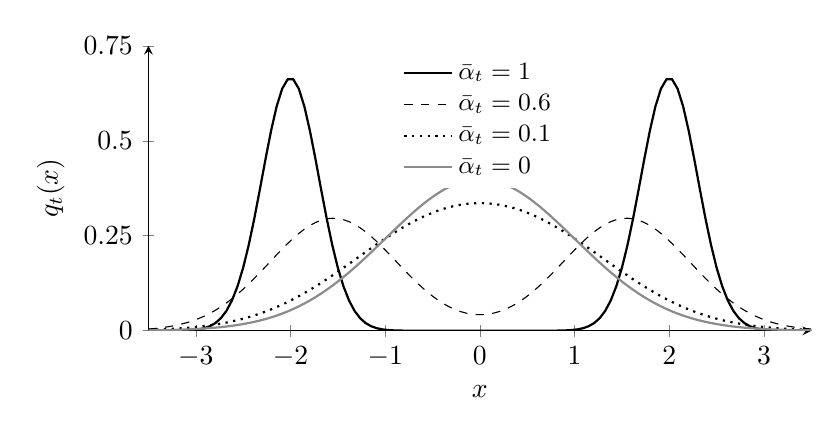
\begin{tikzpicture}
    \begin{axis}[width=10cm, height=5.2cm, domain=-3.5:3.5, samples=120, axis lines=left,
                 xlabel={$x$}, ylabel={$q_t(x)$}, ymin=0, ymax=0.75, ytick={0,0.25,0.5,0.75},
                 legend style={draw=none, font=\small, at={(0.5,0.98)}, anchor=north}, legend cell align=left]
      \addplot[black, thick] {0.5*exp(-(x-2)^2/(2*0.09))/sqrt(2*pi*0.09) + 0.5*exp(-(x+2)^2/(2*0.09))/sqrt(2*pi*0.09)};
      \addlegendentry{$\bar\alpha_t = 1$}
      \addplot[black, dashed] {0.5*exp(-(x-1.549)^2/(2*0.454))/sqrt(2*pi*0.454) + 0.5*exp(-(x+1.549)^2/(2*0.454))/sqrt(2*pi*0.454)};
      \addlegendentry{$\bar\alpha_t = 0.6$}
      \addplot[black, dotted, thick] {0.5*exp(-(x-0.632)^2/(2*0.909))/sqrt(2*pi*0.909) + 0.5*exp(-(x+0.632)^2/(2*0.909))/sqrt(2*pi*0.909)};
      \addlegendentry{$\bar\alpha_t = 0.1$}
      \addplot[black!45, thick] {exp(-x^2/2)/sqrt(2*pi)};
      \addlegendentry{$\bar\alpha_t = 0$}
    \end{axis}
  \end{tikzpicture}
  \caption{Marginals $q_t(x) = \int q(x \mid x_0)\,q(x_0)\,\mathrm{d}x_0$ for data $q(x_0) = \frac12\N(-2, 0.3^2) + \frac12\N(2, 0.3^2)$. By~\eqref{eq:marginal} each mode moves to $\pm 2\sqrt{\bar\alpha_t}$ and its variance grows to $0.09\,\bar\alpha_t + 1 - \bar\alpha_t$.}\label{fig:marginals}
\end{figure}

\section{The reverse process and the variational bound}\label{sec:elbo}
The generative model runs the chain backwards, starting from the prior $p(x_T) = \N(0, I)$:
\begin{equation}\label{eq:reverse}
  p_\theta(x_{0:T}) = p(x_T) \prod_{t=1}^{T} p_\theta(x_{t-1} \mid x_t), \qquad
  p_\theta(x_{t-1} \mid x_t) = \N\!\left(\mu_\theta(x_t, t),\ \sigma_t^2 I\right).
\end{equation}
The variances $\sigma_t^2$ are fixed; only the means are learned~\cite{ho2020}.
The likelihood $p_\theta(x_0)$ integrates over all paths and is intractable, so we maximise a lower bound instead.
Using $q(x_{1:T} \mid x_0)$ as the variational distribution, Jensen's inequality gives
\begin{equation}\label{eq:jensen}
  \log p_\theta(x_0) = \log \E_{q(x_{1:T} \mid x_0)}\!\left[\frac{p_\theta(x_{0:T})}{q(x_{1:T} \mid x_0)}\right]
  \ \ge\ \E_{q}\!\left[\log \frac{p_\theta(x_{0:T})}{q(x_{1:T} \mid x_0)}\right] =: -L .
\end{equation}

\begin{proposition}[Decomposition of the bound]\label{prop:elbo}
The negative bound splits into one term per step:
\begin{equation}\label{eq:elbo}
  L = \underbrace{\KL\!\big(q(x_T \mid x_0)\,\|\,p(x_T)\big)}_{L_T}
    + \sum_{t=2}^{T} \underbrace{\E_{q}\,\KL\!\big(q(x_{t-1} \mid x_t, x_0)\,\|\,p_\theta(x_{t-1} \mid x_t)\big)}_{L_{t-1}}
    \underbrace{-\E_{q} \log p_\theta(x_0 \mid x_1)}_{L_0} .
\end{equation}
\end{proposition}

\begin{proof}
Expand both chains inside the logarithm:
\begin{equation*}
  L = \E_q\!\left[-\log p(x_T) - \sum_{t=1}^{T} \log \frac{p_\theta(x_{t-1} \mid x_t)}{q(x_t \mid x_{t-1})}\right].
\end{equation*}
The forward process is Markov, so $q(x_t \mid x_{t-1}) = q(x_t \mid x_{t-1}, x_0)$, and by Bayes' rule, for $t \ge 2$,
\begin{equation*}
  q(x_t \mid x_{t-1}, x_0) = \frac{q(x_{t-1} \mid x_t, x_0)\, q(x_t \mid x_0)}{q(x_{t-1} \mid x_0)} .
\end{equation*}
The ratios $q(x_t \mid x_0) / q(x_{t-1} \mid x_0)$ telescope over $t = 2, \dots, T$ to $q(x_T \mid x_0) / q(x_1 \mid x_0)$, and the $q(x_1 \mid x_0)$ cancels against the $t = 1$ term. What remains is
\begin{equation*}
  L = \E_q\!\left[\log \frac{q(x_T \mid x_0)}{p(x_T)} + \sum_{t=2}^{T} \log \frac{q(x_{t-1} \mid x_t, x_0)}{p_\theta(x_{t-1} \mid x_t)} - \log p_\theta(x_0 \mid x_1)\right],
\end{equation*}
and each logarithm of a ratio, averaged over $q$, is the KL divergence in~\eqref{eq:elbo}.
\end{proof}

$L_T$ has no parameters and is close to zero when $\abar_T \approx 0$.
Every $L_{t-1}$ compares $p_\theta$ with the \emph{forward posterior} $q(x_{t-1} \mid x_t, x_0)$: the reverse step is trained to match what the forward process implies once the clean $x_0$ is known.
That posterior is Gaussian.

\begin{proposition}[Forward posterior]\label{prop:posterior}
For $t \ge 2$, $q(x_{t-1} \mid x_t, x_0) = \N\!\left(x_{t-1};\ \tilde\mu_t(x_t, x_0),\ \tilde\beta_t I\right)$ with
\begin{equation}\label{eq:posterior}
  \tilde\mu_t(x_t, x_0) = \frac{\sqrt{\abar_{t-1}}\,\beta_t}{1-\abar_t}\,x_0 + \frac{\sqrt{\alpha_t}\,(1-\abar_{t-1})}{1-\abar_t}\,x_t,
  \qquad
  \tilde\beta_t = \frac{1-\abar_{t-1}}{1-\abar_t}\,\beta_t .
\end{equation}
\end{proposition}

\begin{proof}
As a function of $x_{t-1}$, the posterior is proportional to $q(x_t \mid x_{t-1})\, q(x_{t-1} \mid x_0)$, a product of two Gaussians:
\begin{equation*}
  \log q(x_{t-1} \mid x_t, x_0) = -\frac12\left[\frac{\|x_t - \sqrt{\alpha_t}\,x_{t-1}\|^2}{\beta_t} + \frac{\|x_{t-1} - \sqrt{\abar_{t-1}}\,x_0\|^2}{1-\abar_{t-1}}\right] + \text{const}.
\end{equation*}
The coefficient of $-\frac12\|x_{t-1}\|^2$ is the precision
\begin{equation*}
  \frac{\alpha_t}{\beta_t} + \frac{1}{1-\abar_{t-1}} = \frac{\alpha_t(1-\abar_{t-1}) + \beta_t}{\beta_t(1-\abar_{t-1})} = \frac{1-\abar_t}{\beta_t(1-\abar_{t-1})},
\end{equation*}
using $\alpha_t + \beta_t = 1$ and $\alpha_t \abar_{t-1} = \abar_t$. Its inverse is $\tilde\beta_t$.
The linear term is $\big\langle x_{t-1},\ \frac{\sqrt{\alpha_t}}{\beta_t} x_t + \frac{\sqrt{\abar_{t-1}}}{1-\abar_{t-1}} x_0 \big\rangle$, and the mean is $\tilde\beta_t$ times its vector, which is~\eqref{eq:posterior}.
\end{proof}

\section{From the bound to noise prediction}\label{sec:eps}
Both distributions in $L_{t-1}$ are Gaussian with fixed, isotropic variances, so the KL divergence reduces to a squared distance between means:
\begin{equation}\label{eq:kl-means}
  L_{t-1} = \E_q\!\left[\frac{1}{2\sigma_t^2}\,\big\|\tilde\mu_t(x_t, x_0) - \mu_\theta(x_t, t)\big\|^2\right] + C .
\end{equation}
The network could predict $\tilde\mu_t$ directly, but a better target comes from rewriting it in terms of the noise.
Solving~\eqref{eq:marginal} for $x_0 = (x_t - \sqrt{1-\abar_t}\,\epsilon)/\sqrt{\abar_t}$ and substituting into~\eqref{eq:posterior}, the coefficient of $x_t$ becomes $\frac{\beta_t + \alpha_t(1-\abar_{t-1})}{(1-\abar_t)\sqrt{\alpha_t}} = \frac{1}{\sqrt{\alpha_t}}$, and so
\begin{equation}\label{eq:mu-eps}
  \tilde\mu_t = \frac{1}{\sqrt{\alpha_t}}\left(x_t - \frac{\beta_t}{\sqrt{1-\abar_t}}\,\epsilon\right).
\end{equation}
Since $x_t$ is the network's input, the only unknown in~\eqref{eq:mu-eps} is $\epsilon$. We therefore let the network predict it,
\begin{equation}\label{eq:mu-theta}
  \mu_\theta(x_t, t) = \frac{1}{\sqrt{\alpha_t}}\left(x_t - \frac{\beta_t}{\sqrt{1-\abar_t}}\,\epsilon_\theta(x_t, t)\right),
\end{equation}
and~\eqref{eq:kl-means} becomes a weighted denoising objective:
\begin{equation}\label{eq:weighted}
  L_{t-1} = \E_{x_0, \epsilon}\!\left[\frac{\beta_t^2}{2\sigma_t^2\,\alpha_t\,(1-\abar_t)}\,
  \big\|\epsilon - \epsilon_\theta\big(\sqrt{\abar_t}\,x_0 + \sqrt{1-\abar_t}\,\epsilon,\ t\big)\big\|^2\right] + C .
\end{equation}
Ho et al.~\cite{ho2020} found that dropping the weight and sampling $t$ uniformly trains better samplers:
\begin{equation}\label{eq:simple}
  L_{\text{simple}}(\theta) = \E_{t \sim \mathcal{U}\{1, \dots, T\},\ x_0,\ \epsilon}\,\big\|\epsilon - \epsilon_\theta\big(\sqrt{\abar_t}\,x_0 + \sqrt{1-\abar_t}\,\epsilon,\ t\big)\big\|^2 .
\end{equation}
Relative to the bound, this puts more weight on large $t$, where the denoising task is hardest.
Predicting $\epsilon$ is one of three equivalent choices; Table~\ref{tab:param} lists them.

\begin{table}[t]
  \centering
  \caption{Three parameterisations of the reverse mean. Each is an affine function of the others given $x_t$, so they differ only in how the loss weights the time steps.}\label{tab:param}
  \begin{tabular}{lll}
    \toprule
    Network predicts & Reverse mean $\mu_\theta(x_t, t)$ & Relation \\
    \midrule
    Noise $\epsilon_\theta$ & $\frac{1}{\sqrt{\alpha_t}}\big(x_t - \frac{\beta_t}{\sqrt{1-\bar\alpha_t}}\epsilon_\theta\big)$ & --- \\
    Clean data $\hat x_\theta$ & $\tilde\mu_t(x_t, \hat x_\theta)$ from~\eqref{eq:posterior} & $\hat x_\theta = \frac{x_t - \sqrt{1-\bar\alpha_t}\,\epsilon_\theta}{\sqrt{\bar\alpha_t}}$ \\
    Score $s_\theta$ & $\frac{1}{\sqrt{\alpha_t}}\big(x_t + \beta_t\, s_\theta\big)$ & $s_\theta = -\frac{\epsilon_\theta}{\sqrt{1-\bar\alpha_t}}$ \\
    \bottomrule
  \end{tabular}
\end{table}

\section{Noise prediction is score estimation}\label{sec:score}
The last row of Table~\ref{tab:param} is more than a change of variables: the optimal noise predictor is the score of the noisy marginal $q_t(x) = \int q(x \mid x_0)\,q(x_0)\,\mathrm{d}x_0$.

\begin{proposition}[Tweedie's formula]\label{prop:tweedie}
The minimiser of~\eqref{eq:simple} at step $t$ is
\begin{equation}\label{eq:tweedie}
  \epsilon^*(x_t, t) = -\sqrt{1-\abar_t}\;\nabla_{x_t} \log q_t(x_t),
\end{equation}
or equivalently, in terms of the clean data,
\begin{equation}\label{eq:tweedie-x0}
  \E[x_0 \mid x_t] = \frac{x_t + (1-\abar_t)\,\nabla_{x_t} \log q_t(x_t)}{\sqrt{\abar_t}} .
\end{equation}
\end{proposition}

\begin{proof}
A squared-error loss is minimised by the conditional mean, so $\epsilon^*(x_t, t) = \E[\epsilon \mid x_t]$.
Differentiating $q_t(x_t) = \int q(x_t \mid x_0)\,q(x_0)\,\mathrm{d}x_0$ under the integral and dividing by $q_t(x_t)$ gives
\begin{equation*}
  \nabla_{x_t} \log q_t(x_t) = \int \frac{q(x_t \mid x_0)\,q(x_0)}{q_t(x_t)}\,\nabla_{x_t} \log q(x_t \mid x_0)\,\mathrm{d}x_0
  = \E\big[\nabla_{x_t} \log q(x_t \mid x_0) \,\big|\, x_t\big].
\end{equation*}
By Proposition~\ref{prop:marginal}, $\nabla_{x_t} \log q(x_t \mid x_0) = -(x_t - \sqrt{\abar_t}\,x_0)/(1-\abar_t) = -\epsilon/\sqrt{1-\abar_t}$.
Taking the conditional expectation gives~\eqref{eq:tweedie}, and~\eqref{eq:tweedie-x0} follows by taking $\E[\,\cdot \mid x_t]$ of~\eqref{eq:marginal}.
\end{proof}

So training with~\eqref{eq:simple} is denoising score matching~\cite{vincent2011} at every noise level at once, and $s_\theta = -\epsilon_\theta/\sqrt{1-\abar_t}$ estimates $\nabla \log q_t$.
This is the bridge to score-based generative models~\cite{song2019}; \eqref{eq:tweedie-x0} is Tweedie's formula~\cite{efron2011}.

\section{Training and sampling}\label{sec:algorithms}
Training (Algorithm~\ref{alg:train}) is plain regression onto the noise.
Sampling (Algorithm~\ref{alg:sample}) runs the reverse chain~\eqref{eq:reverse} with the mean~\eqref{eq:mu-theta}.
Both $\sigma_t^2 = \beta_t$ and $\sigma_t^2 = \tilde\beta_t$ work well in practice: they are the optimal choices when $x_0 \sim \N(0, I)$ and when $x_0$ is a single point, respectively~\cite{ho2020}.

\begin{algorithm}[t]
  \caption{Training}\label{alg:train}
  \begin{algorithmic}[1]
    \Repeat
      \State $x_0 \sim q(x_0)$, \quad $t \sim \mathcal{U}\{1, \dots, T\}$, \quad $\epsilon \sim \N(0, I)$
      \State $x_t \gets \sqrt{\bar\alpha_t}\,x_0 + \sqrt{1-\bar\alpha_t}\,\epsilon$ \Comment{Proposition~\ref{prop:marginal}}
      \State take a gradient step on $\nabla_\theta \|\epsilon - \epsilon_\theta(x_t, t)\|^2$
    \Until{converged}
  \end{algorithmic}
\end{algorithm}

\begin{algorithm}[t]
  \caption{Ancestral sampling}\label{alg:sample}
  \begin{algorithmic}[1]
    \State $x_T \sim \N(0, I)$
    \For{$t = T, \dots, 1$}
      \State $z \sim \N(0, I)$ if $t > 1$, else $z = 0$
      \State $x_{t-1} \gets \frac{1}{\sqrt{\alpha_t}}\big(x_t - \frac{\beta_t}{\sqrt{1-\bar\alpha_t}}\,\epsilon_\theta(x_t, t)\big) + \sigma_t z$ \Comment{mean~\eqref{eq:mu-theta}}
    \EndFor
    \State \Return $x_0$
  \end{algorithmic}
\end{algorithm}

In code, one training step is a few lines:
\begin{lstlisting}[language=python]
def loss(eps_model, x0, alpha_bar):              # alpha_bar: tensor of shape [T]
    t = torch.randint(0, len(alpha_bar), (x0.shape[0],), device=x0.device)
    a = alpha_bar[t].view(-1, *[1] * (x0.dim() - 1))
    eps = torch.randn_like(x0)
    xt = a.sqrt() * x0 + (1 - a).sqrt() * eps    # Proposition 1
    return (eps - eps_model(xt, t)).pow(2).mean()
\end{lstlisting}

\section{Deterministic sampling}\label{sec:ddim}
Nothing in $L_{\text{simple}}$ depends on the joint forward process: it only uses the marginals $q(x_t \mid x_0)$.
Any process with the same marginals therefore shares the same trained network.
Song et al.~\cite{song2021ddim} construct a family of non-Markovian ones, indexed by $\sigma_t \ge 0$, whose reverse step is
\begin{equation}\label{eq:ddim}
  x_{t-1} = \sqrt{\abar_{t-1}}\;\hat x_0
  + \sqrt{1-\abar_{t-1}-\sigma_t^2}\;\epsilon_\theta(x_t, t) + \sigma_t z,
  \qquad
  \hat x_0 = \frac{x_t - \sqrt{1-\abar_t}\,\epsilon_\theta(x_t, t)}{\sqrt{\abar_t}} .
\end{equation}
The step reads naturally: estimate the clean sample, then re-noise it to level $t-1$ using the predicted noise direction.
With $\sigma_t^2 = \tilde\beta_t$ this is exactly Algorithm~\ref{alg:sample}.
With $\sigma_t = 0$ the sampler is deterministic (DDIM). It maps each $x_T$ to one $x_0$, and it can skip steps, since~\eqref{eq:ddim} only needs $\abar$ at the two levels involved.

\section{The continuous-time limit}\label{sec:sde}
Let the steps shrink: $t \in [0, 1]$, $\beta_t = \beta(t)\,\Delta t$.
One forward step is then, to first order in $\Delta t$,
\begin{equation*}
  x_{t+\Delta t} = \sqrt{1-\beta(t)\Delta t}\;x_t + \sqrt{\beta(t)\Delta t}\;\epsilon
  \approx x_t - \tfrac12 \beta(t)\,x_t\,\Delta t + \sqrt{\beta(t)}\,\sqrt{\Delta t}\,\epsilon ,
\end{equation*}
which is the Euler--Maruyama discretisation of the variance-preserving SDE~\cite{song2021sde}
\begin{equation}\label{eq:vp-sde}
  \mathrm{d}x = -\tfrac12 \beta(t)\,x\,\mathrm{d}t + \sqrt{\beta(t)}\,\mathrm{d}w .
\end{equation}
Anderson's theorem~\cite{anderson1982} gives its time reversal, which again needs only the score:
\begin{equation}\label{eq:reverse-sde}
  \mathrm{d}x = \Big[-\tfrac12 \beta(t)\,x - \beta(t)\,\nabla_x \log q_t(x)\Big]\mathrm{d}t + \sqrt{\beta(t)}\,\mathrm{d}\bar w .
\end{equation}
Replacing the score with $s_\theta = -\epsilon_\theta/\sqrt{1-\abar_t}$ (Proposition~\ref{prop:tweedie}) and discretising~\eqref{eq:reverse-sde} recovers ancestral sampling to first order in $\Delta t$.
Dropping the noise and halving the score term gives the \emph{probability-flow ODE}
$\mathrm{d}x = -\tfrac12 \beta(t)\,\big[x + \nabla_x \log q_t(x)\big]\,\mathrm{d}t$, whose solutions have the same marginals $q_t$ as~\eqref{eq:vp-sde}. DDIM ($\sigma_t = 0$) can be read as a discretisation of this ODE~\cite{song2021ddim}.

\section{Choosing the schedule}\label{sec:schedule}
Everything above depends on the schedule only through $\abar_t$, the fraction of signal variance left at step $t$.
Equivalently, it depends through the signal-to-noise ratio $\mathrm{SNR}(t) = \abar_t / (1-\abar_t)$, which is all the continuous-time bound depends on~\cite{kingma2021}.
The original linear schedule~\cite{ho2020} increases $\beta_t$ from $10^{-4}$ to $0.02$ over $T = 1000$ steps.
It destroys most of the signal well before the end, so the last few hundred steps are spent on nearly pure noise.
The cosine schedule~\cite{nichol2021}, $\abar_t = f(t)/f(0)$ with $f(t) = \cos^2\!\big(\frac{t/T + s}{1 + s}\cdot\frac{\pi}{2}\big)$ and $s = 0.008$, decays more evenly (Figure~\ref{fig:schedule}).

\begin{figure}[t]
  \centering
  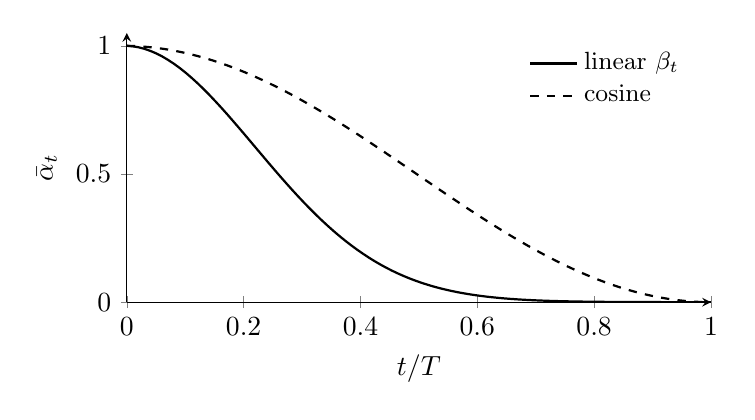
\begin{tikzpicture}
    \begin{axis}[width=9cm, height=5cm, domain=0:1, samples=100, axis lines=left,
                 xlabel={$t/T$}, ylabel={$\bar\alpha_t$}, ymin=0, ymax=1.05,
                 legend style={draw=none, font=\small}, legend pos=north east, legend cell align=left]
      \addplot[black, thick] {exp(-0.1*x - 9.95*x^2)};
      \addlegendentry{linear $\beta_t$}
      \addplot[black, thick, dashed] {cos(deg((x + 0.008)/1.008*pi/2))^2 / cos(deg(0.008/1.008*pi/2))^2};
      \addlegendentry{cosine}
    \end{axis}
  \end{tikzpicture}
  \caption{$\bar\alpha_t$ under the two schedules ($T = 1000$). For the linear schedule, $\bar\alpha_t \approx \exp\!\big(-\sum_{s \le t} \beta_s\big) = e^{-0.1u - 9.95u^2}$ with $u = t/T$.}\label{fig:schedule}
\end{figure}

\section{Summary}\label{sec:summary}
The derivation is a short chain of exact steps.
The forward marginals are Gaussian in closed form~\eqref{eq:marginal}, and the bound splits into Gaussian KLs~\eqref{eq:elbo}.
Each KL compares the model with a Gaussian posterior~\eqref{eq:posterior}, whose mean is an affine function of the noise~\eqref{eq:mu-eps}.
Regressing the noise~\eqref{eq:simple} therefore fits every reverse step, and by Tweedie's formula (Proposition~\ref{prop:tweedie}) it also estimates the score.
The score is the only learned quantity that ancestral sampling, DDIM and the reverse SDE need.

\begin{thebibliography}{10}
  \bibitem{sohl2015} J. Sohl-Dickstein, E. Weiss, N. Maheswaranathan, S. Ganguli. Deep unsupervised learning using nonequilibrium thermodynamics. In \emph{ICML}, 2015.
  \bibitem{ho2020} J. Ho, A. Jain, P. Abbeel. Denoising diffusion probabilistic models. In \emph{NeurIPS}, 2020.
  \bibitem{song2019} Y. Song, S. Ermon. Generative modeling by estimating gradients of the data distribution. In \emph{NeurIPS}, 2019.
  \bibitem{song2021sde} Y. Song, J. Sohl-Dickstein, D. P. Kingma, A. Kumar, S. Ermon, B. Poole. Score-based generative modeling through stochastic differential equations. In \emph{ICLR}, 2021.
  \bibitem{vincent2011} P. Vincent. A connection between score matching and denoising autoencoders. \emph{Neural Computation}, 23(7):1661--1674, 2011.
  \bibitem{efron2011} B. Efron. Tweedie's formula and selection bias. \emph{Journal of the American Statistical Association}, 106(496):1602--1614, 2011.
  \bibitem{song2021ddim} J. Song, C. Meng, S. Ermon. Denoising diffusion implicit models. In \emph{ICLR}, 2021.
  \bibitem{anderson1982} B. D. O. Anderson. Reverse-time diffusion equation models. \emph{Stochastic Processes and their Applications}, 12(3):313--326, 1982.
  \bibitem{kingma2021} D. P. Kingma, T. Salimans, B. Poole, J. Ho. Variational diffusion models. In \emph{NeurIPS}, 2021.
  \bibitem{nichol2021} A. Q. Nichol, P. Dhariwal. Improved denoising diffusion probabilistic models. In \emph{ICML}, 2021.
\end{thebibliography}
